\documentclass[border=3pt]{standalone}
% Preâmbulo compartilhado pelos diagramas TikZ da aula 6 de IHC (Necessidades e Requisitos)
\usepackage[T1]{fontenc}
\usepackage[utf8]{inputenc}
\usepackage{lmodern}
\usepackage{amsmath}
\usepackage{xcolor}
\usepackage{tikz}
\usetikzlibrary{arrows.meta,angles,quotes,decorations.pathmorphing,calc,
                positioning,shapes.geometric,shapes.misc,backgrounds,fit,
                math}

% Paleta (mesma dos SVGs originais)
% Paleta da disciplina de IHC: acento roxo (#755099), da capa do livro.
% (o nome "dblue" é mantido para não alterar todos os diagramas)
\definecolor{dblue}{HTML}{755099}
\definecolor{dorange}{HTML}{B3541E}
\definecolor{dgreen}{HTML}{4A7C59}
\definecolor{dred}{HTML}{9C4B4B}
\definecolor{dcream}{HTML}{F4F1EA}
\definecolor{dshade}{HTML}{DDD7C9}

% Função gaussiana (não normalizada por padrão de escala visual)
\pgfmathdeclarefunction{gauss}{3}{%
  \pgfmathparse{1/(#3*sqrt(2*pi))*exp(-((#1-#2)^2)/(2*#3^2))}%
}

% Estilos comuns (prefixo d... para não colidir com chaves internas do pgf)
\tikzset{
  >={Stealth[length=2mm]},
  dguide/.style={gray!55, dashed, line width=0.4pt},
  daxis/.style={gray!60, line width=0.7pt, ->},
  dbody/.style={fill=black!3, draw=black!80, line width=1pt},
  dacc/.style={draw=dblue, line width=1pt},
  dlbl/.style={black!55, font=\small},
  dsub/.style={black!45, font=\footnotesize},
  dstate/.style={circle, draw=black!80, fill=dcream, line width=1pt,
                 minimum size=17mm, font=\large, inner sep=1pt},
  dobs/.style={circle, draw=black!80, fill=dshade, line width=1pt,
               minimum size=14mm, font=\large, inner sep=1pt},
  dbox/.style={rounded corners=2pt, draw=black!80, fill=dcream, line width=1pt,
               align=center, inner sep=6pt},
  dop/.style={circle, draw=black!80, fill=white, line width=1pt,
              minimum size=6mm, inner sep=0pt, font=\small},
  dtrans/.style={->, dblue, line width=1pt},
  dmeas/.style={->, dorange, line width=1pt},
  dcurve/.style={line width=1pt, dblue},
  dcurveb/.style={line width=1.4pt, dorange},
}

\begin{document}
\hyphenpenalty=10000 \exhyphenpenalty=10000 \tolerance=9999 \emergencystretch=3em
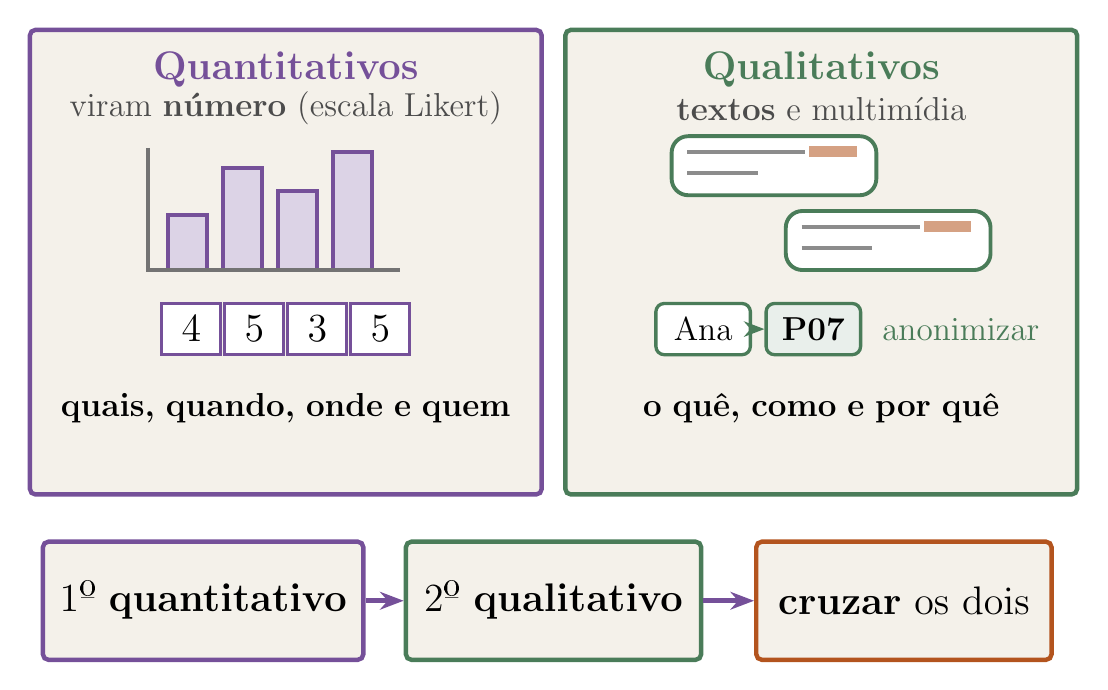
\begin{tikzpicture}[x=1cm,y=1cm]
\node[dbox, draw=dblue, line width=1.6pt, minimum width=6.5cm, minimum height=5.9cm] at (3.25,5.35) {};
\node[font=\Large\bfseries, dblue] at (3.25,7.80) {Quantitativos};
\node[font=\large, black!70] at (3.25,7.30) {viram \textbf{número} (escala Likert)};
\draw[dblue, fill=dblue!25!white, line width=1.4pt] (1.75,5.25) rectangle ++(0.5,0.70);
\draw[dblue, fill=dblue!25!white, line width=1.4pt] (2.45,5.25) rectangle ++(0.5,1.30);
\draw[dblue, fill=dblue!25!white, line width=1.4pt] (3.15,5.25) rectangle ++(0.5,1.00);
\draw[dblue, fill=dblue!25!white, line width=1.4pt] (3.85,5.25) rectangle ++(0.5,1.50);
\draw[black!55, line width=1.3pt] (1.50,6.80) -- (1.50,5.25) -- (4.70,5.25);
\node[font=\large, black!65, anchor=east] at (1.35,5.35) {};
\node[draw=dblue, fill=white, line width=1.2pt, minimum width=0.75cm, minimum height=0.65cm, font=\Large] at (2.05,4.50) {4};
\node[draw=dblue, fill=white, line width=1.2pt, minimum width=0.75cm, minimum height=0.65cm, font=\Large] at (2.85,4.50) {5};
\node[draw=dblue, fill=white, line width=1.2pt, minimum width=0.75cm, minimum height=0.65cm, font=\Large] at (3.65,4.50) {3};
\node[draw=dblue, fill=white, line width=1.2pt, minimum width=0.75cm, minimum height=0.65cm, font=\Large] at (4.45,4.50) {5};
\node[font=\large, text width=6.1cm, align=center] at (3.25,3.50) {\textbf{quais, quando, onde e quem}};
\node[dbox, draw=dgreen, line width=1.6pt, minimum width=6.5cm, minimum height=5.9cm] at (10.05,5.35) {};
\node[font=\Large\bfseries, dgreen] at (10.05,7.80) {Qualitativos};
\node[font=\large, black!70] at (10.05,7.30) {\textbf{textos} e multimídia};
\draw[dgreen, fill=white, line width=1.4pt, rounded corners=6pt] (8.15,6.20) rectangle ++(2.60,0.75);
\draw[black!45, line width=1.3pt] (8.35,6.75) -- ++(1.5,0) (8.35,6.48) -- ++(0.9,0);
\fill[dorange!55!white] (9.90,6.68) rectangle ++(0.6,0.14);
\draw[dgreen, fill=white, line width=1.4pt, rounded corners=6pt] (9.60,5.25) rectangle ++(2.60,0.75);
\draw[black!45, line width=1.3pt] (9.80,5.80) -- ++(1.5,0) (9.80,5.53) -- ++(0.9,0);
\fill[dorange!55!white] (11.35,5.73) rectangle ++(0.6,0.14);
\node[draw=dgreen, fill=white, line width=1.2pt, rounded corners=3pt, font=\large, minimum height=0.65cm, minimum width=1.2cm] (a) at (8.55,4.50) {Ana};
\node[draw=dgreen, fill=dgreen!12!white, line width=1.2pt, rounded corners=3pt, font=\large\bfseries, minimum height=0.65cm, minimum width=1.2cm] (b) at (9.95,4.50) {P07};
\draw[dgreen, line width=1.6pt, -{Stealth[length=2.6mm]}] (a) -- (b);
\node[font=\large, dgreen, anchor=west] at (10.70,4.50) {anonimizar};
\node[font=\large, text width=6.1cm, align=center] at (10.05,3.50) {\textbf{o quê, como e por quê}};
\node[dbox, draw=dblue, line width=1.6pt, minimum width=3.75cm, minimum height=1.5cm, font=\Large] (f0) at (2.20,1.05) {1º \textbf{quantitativo}};
\node[dbox, draw=dgreen, line width=1.6pt, minimum width=3.75cm, minimum height=1.5cm, font=\Large] (f1) at (6.65,1.05) {2º \textbf{qualitativo}};
\draw[dtrans, line width=1.8pt, -{Stealth[length=3mm]}] (f0.east) -- (f1.west);
\node[dbox, draw=dorange, line width=1.6pt, minimum width=3.75cm, minimum height=1.5cm, font=\Large] (f2) at (11.10,1.05) {\textbf{cruzar} os dois};
\draw[dtrans, line width=1.8pt, -{Stealth[length=3mm]}] (f1.east) -- (f2.west);
\end{tikzpicture}
\end{document}
